\documentclass[a4paper,twoside,phd]{BYUPhys}
% The BYUPhys class is for producing theses and dissertations
% in the BYU Department of Physics and Astronomy.  You can supply
% the following optional arguments in the square brackets to
% specify the thesis type:
%
%   senior  : Produces the senior thesis preliminary pages (default)
%   honors  : Produces the honors thesis preliminary pages
%   masters : Produces the masters thesis preliminary pages
%   phd     : Produces the PhD dissertation preliminary pages
%
% The default format is appropriate for printing, with blank pages
% inserted after the preliminary pages in twoside mode so you can
% send it directly to a two-sided printer. However, for ETD
% submission the blank pages need to be removed from the final output.
% The following option does this for you:
%
%   etd     : Produces a copy with no blank pages in the preliminary section.
%             Remove this option to produce a version with blank pages inserted
%             for easy double sided printing.
%
% The rest of the class options are the same as the regular book class.
% A few to remember:
%
%   oneside : Produces single sided print layout (recommended for theses less than 50 pages)
%   twoside : Produces double sided print layout (the default if you remove oneside)
%
% The BYUPhys class provides the following macros:
%
%   \makepreliminarypages : Makes the preliminary pages
%   \clearemptydoublepage : same as \cleardoublepage but doesn't put page numbers
%                           on blank intervening pages
%   \singlespace          : switch to single spaced lines
%   \doublespace          : switch to double spaced lines
%
% --------------------------- Load Packages ---------------------------------

% The graphicx package allows the inclusion of figures.  Plain LaTeX and
% pdfLaTeX handle graphics differently. The following code checks which one
% you are compiling with, and switches the graphicx package options accordingly.
\usepackage{ifpdf}
\ifpdf
  \usepackage[pdftex]{graphicx}
\else
  \usepackage[dvips]{graphicx}
\fi

%%%%%%%%%%%%%%%%%%%%%%%%%%%%%%%%%%%%%%%%%%%%%%%%%%%%%%%%%%%%%%%%%%
% Edited : Beeshanga
%
% If you need to include any code in the text use this package
% \usepackage{listings}
% It can be used to make key words bold, add colours, etc. Refer
% to http://en.wikibooks.org/wiki/LaTeX/Packages/Listings for
% more information.
%
% For theorems, propositions, proofs and assumtions use this
% package
% \usepackage{amsthm}
% For more information refer to the following website
% http://en.wikibooks.org/wiki/LaTeX/Theorems
%
%%%%%%%%%%%%%%%%%%%%%%%%%%%%%%%%%%%%%%%%%%%%%%%%%%%%%%%%%%%%%%%%%%

% The fancyhdr package allows you to easily customize the page header.
% The settings below produce a nice, well separated header.
\usepackage{fancyhdr}
  \fancyhead{}
  \fancyhead[LO]{\slshape \rightmark}
  \fancyhead[RO,LE]{\textbf{\thepage}}
  \fancyhead[RE]{\slshape \leftmark}
  \fancyfoot{}
  \pagestyle{fancy}
  \renewcommand{\chaptermark}[1]{\markboth{\chaptername \ \thechapter. #1}{}}
  \renewcommand{\sectionmark}[1]{\markright{\thesection \ #1}}


% The cite package cleans up the way citations are handled.  For example, it
% changes the citation [1,2,3,6,7,8,9,10,11] into [1-3,6-11].  If your advisor
% wants superscript citations, use the overcite package instead of the cite package.
\usepackage{cite}

% The makeidx package makes your index for you.  To make an index entry,
% go to the place in the book that should be referenced and type
%  \index{key}
% An index entry labeled "key" (or whatever you type) will then
% be included and point to the correct page.
%\usepackage{makeidx}
%\makeindex

% The url package allows for the nice typesetting of URLs.  Since URLs are often
% long with no spaces, they mess up line wrapping.  The command \url{http://www.physics.byu.edu}
% allows LaTeX to break the url across lines at appropriate places: e.g. http://www.
% physics.byu.edu.  This is helpful if you reference web pages.
\usepackage{url}
\urlstyle{rm}

% If you have a lot of equations, you might be interested in the amstex package.
% It defines a number of environments and macros that are helpful for mathematics.
% We don't do much math in this example, so we haven't used amstex here.
\usepackage{amsmath}
\usepackage{amssymb}
\usepackage{subfigure}
\usepackage{cite}
\usepackage{amsxtra}
\usepackage{amsfonts}
\usepackage{graphicx}
\usepackage{multirow} % This is package for multi-rows in tables added on 7th July 2009 by Arif
%\usepackage{setspace}

% The caption package allows us to change the formatting of figure captions.
% The commands here change to the suggested caption format: single spaced and a bold tag
\usepackage[labelfont=bf,labelsep=colon]{caption}%[2008/04/01]
 \DeclareCaptionFormat{suggested}{\singlespace#1#2#3\par\doublespace}
 \captionsetup{format=suggested}


\usepackage{array}
\usepackage{multirow}
\usepackage{verbatim}
\usepackage{enumerate}

% Defining the symbols




% The hyperref package provides automatic linking and bookmarking for the table
% of contents, index, equation references, and figure references.  It must be
% included for the BYU Physics class to make a properly functioning electronic
% thesis.  It should be the last package loaded if possible.
%
% To include a link in your pdf use \href{URL}{Text to be displayed}.  If your
% display text is the URL, you probably should use the \url{} command discussed
% above.
%
% To add a bookmark in the pdf you can use \pdfbookmark.  You can look up its usage
% in the hyperref package documentation
\usepackage[bookmarksnumbered,pdfpagelabels=true,plainpages=false,colorlinks=true,
            linkcolor=black,citecolor=red,urlcolor=blue]{hyperref}

% ------------------------- Fill in these fields for the preliminary pages ----------------------------
%
% For Senior and honors this is the year and month that you submit the thesis
% For Masters and PhD, this is your graduation date
  \Year{2018}
  \Month{November XX,}
  \Author{Dione Morales}

% If you have a long title, split it between two lines. The \TitleBottom field defines the second line
% A two line title should be an "inverted pyramid" with the top line longer than the bottom.
  \TitleTop{Detecting health misinformation in web page text}
  \TitleBottom{using deep learning methods}
  %\TitleBottom{Line 2 of the Tile} % edited Beeshanga
 \DegreeTitle{Bachelor of Engineering
 \\ Computer Engineering Stream} % edited Beeshanga

% Your research advisor
 \Advisor{Supervisor: Associate Professor Adam Dunn}

% The department undergraduate research coordinator
%  \UgradCoord{A}

% The representative of the department who will approve your thesis (usually the chair)
%  \DepRep{B}

% Acknowledge those who helped and supported you

  \Acknowledgments{
  \vspace{-1.5cm}
    \noindent I would like to acknowledge ...

  }


% The title of the department representative
%  \DepRepTitle{Chair}
  \Statement{
    \noindent I, (insert name here), declare that this report, submitted as part of the requirement for the award of Bachelor of Engineering in the School of Engineering, Macquarie University, is entirely my own work unless otherwise referenced or acknowledged. This document has not been submitted for qualification or assessment an any academic institution.
    \vspace{0.5cm}

    \noindent     Student's Name:

    \vspace{0.25cm}

    \noindent Student's Signature:

    \vspace{0.25cm}

    \noindent     Date:
    }

% The text of your abstract
\Abstract{
\vspace{-1.5 cm}
This is where you write your abstract ...

}



% Statement of Candidate



\fussy

\begin{document}

 % Start page counting in roman numerals
 \frontmatter

 % This command makes the formal preliminary pages.
 % You can comment it out during the drafting process if you want to save paper.

 \makepreliminarypages


%\clearemptydoublepage
\doublespace
%\include{Publications/publications}

% \clearemptydoublepage
%\include{Organization/organization}

 \clearemptydoublepage
\singlespace
 % Make the table of contents.
 \tableofcontents

\clearemptydoublepage
% Make the list of figures
\listoffigures

\clearemptydoublepage
% Make the list of tables
\listoftables

\clearemptydoublepage

% Start regular page counting at page 1
\mainmatter
%
\chapter{Introduction}
\label{chap:Introduction}

Why we should care about minimizing the spread of misinformation online:
\begin{itemize}
	\item The large amount of information being passed around today (where a large majority of the content being shared is not verified). This is largely due to the ubiquity of social network sites (SNS) today whose main function is to spread information, factual or not.
	
	\item Information that is classified to be as rumors tend to generally have more reach than non-rumor based information (3x more shares)
	
	\item With the increase prevalence of social media, popular users and communities are capable of spreading factually incorrect content as they are generally not expected to filter the content they share based on its factual accuracy 
	
	\item The increase use of 'trending', 'discover' etc. sections that encourage users to post content that aim to maximize the number of clicks their content receive rather than the accuracy and reliability of the content
	
\end{itemize}





\section{Project Goal}

This project aims to...

\begin{itemize}
	\item Evaluate the performance of general fake news classifiers on domain specific health related online content.
	\item EITHER investigate the effectiveness of attention based mechanisms in explaining the underlying workings of the fake news classifiers developed OR
	\item Investigate the effectiveness of the application of transfer learning methods on the general fake news classifiers.
\end{itemize}

\section{Project Planning}
Introduction for this section

\subsection{Project Scope}
The scope of project

\subsection{Project Timeline}
When things should be done by

\subsection{Project Cost}
Expected cost of the project




\chapter{Background and Related Work}
\label{chap:LitReview}

\section{Things to cover}
\begin{itemize}
	\item Previous approaches (e.g. NLP, ML) and what they lacked
	\item Deep Learning background info
	\item Deep learning based approaches
	\item How attention or transfer learning works
	\item Fake news challenge top 4 solutions
\end{itemize}



\section{Prior Approaches}
\label{sec:CapResultsReview}

In a

\begin{figure}[t]
\centering
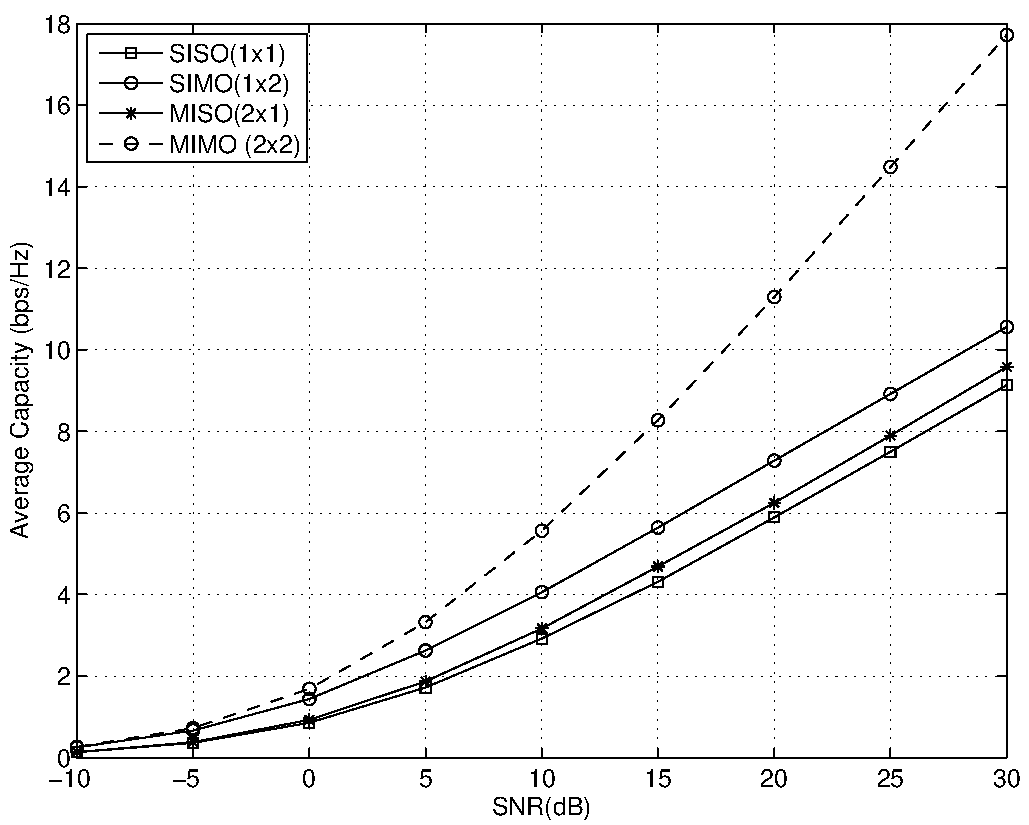
\includegraphics[width=8cm]{cap1}
\caption{Comparison of capacity for single and multiple antenna systems.}
\label{fig:cap1}
\end{figure}

\

\subsubsection{Channel Knowledge at the Base Station}

The channel.

\subsubsection{MAC-BC Duality}

In order to find an a
\chapter{User Selection in MIMO Broadcast Channels}
\label{chap:singleuser}

\section{Introduction \label{sec:Intro-ChapUserSelec}}

\begin{itemize}

\item We identify the limitations of current algorithms and situations where these algorithms are suboptimal.

\item We propose modifications of user selection algorithms that reduce execution complexity but retain efficiency.

\item We develop analytical bounds to show that the proposed algorithms are asymptotically effective.

\item We compare the performance of the proposed user selection algorithms with the current user selection algorithms under both DPC and ZF precoding techniques.

\item We show that the proposed user selection algorithms reduce the computational complexity while retaining a high degree of effectiveness in terms of sum-capacity, as compared to other user selection algorithms, under both precoding techniques.

\end{itemize}


This chapter is organised as follows. Section \ref{sect:RelWorksingle-user} presents work related to this chapter. In Section \ref{sect:chap2sysmodel}, the system model is described. Section \ref{sect:precoding} describes precoding techniques. Section \ref{sect:sus} is devoted to the proposed user selection algorithms and presents the analytical bounds on the sum-capacity of the proposed user selection algorithms. Performance analysis of different user selection algorithms along with the proposed user selection algorithms is presented in Section \ref{sect:simresults}. Finally, Section \ref{sect:conc3} concludes the chapter.

\section{Related Work \label{sect:RelWorksingle-user}}

In this section, we review some current user selection algorithms for MIMO broadcast wireless channels.


A user select.

\section{System Model \label{sect:chap2sysmodel}}

We now consider a


This chapter examined current user selection \cite{andrews05} algorithms for wireless broadcast channels. It compared the performance of the algorithms, identified situations where they were suboptimal and developed modifications to reduce computation time without reducing effectiveness. In particular, we presented a modified user selection algorithm, and then two variants were developed that could be used for both ZF and DPC precoding. It was shown that the proposed algorithms work reasonably well compared to other user selection algorithms. The modifications were tested and suggestions for setting parameters were made.

\chapter{Conclusions and Future Work}
\label{chap:Conclusions}


\section{Conclusions}
\label{sec:ConclusionsConclusions}

This



\clearemptydoublepage
\chapter{Abbreviations}
\label{chap:abbreviations}

\begin{tabbing}

AWGN \qquad \qquad \= Additive White Gaussian Noise\\
BC \> Broadcast Channel\\
BS \> Base Station\\
CSI \> Channel State Information\\
CSIR \> Channel State Information at Receiver\\
CSIT \> Channel State Information at Transmitter\\
dB \> Decibels\\
DPC \> Dirty Paper Coding\\
GS \> Gram-Schmidt\\
RVQ \> Random Vector Quantisation\\
SISO \> Single Input Single Output\\
SNR \> Signal to Noise Ratio\\
SINR \> Signal to Interference plus Noise Ratio\\
MISO \> Multiple Input Single Output\\
SIMO \> Single Input Multiple Output\\
MIMO \> Multiple Input Multiple Output\\
MMSE \> Minimum Mean Square Error\\
MRC \> Maximum Ratio Combining\\
QoS \> Quality of Service\\
TDD \> Time Division Duplex\\
FDD \> Frequency Division Duplex\\
ZF \> Zero-Forcing\\
ZFBF \> Zero-Forcing Beamforming\\
ZMCSCG \> Zero Mean Circularly Symmetric Complex Gaussian\\

\end{tabbing}

%\phantomsection \addcontentsline{toc}{chapter}{Index}
% \renewcommand{\baselinestretch}{1} \small \normalsize
% \printindex

\appendix
\chapter{name of appendix A}
\section{Overview}
here is the Overview of appendix A ...
\section{Name of this section}
here is the content of this section ...
\chapter{name of appendix B}
\section{Overview}
here is the Overview of appendix B ...
\section{Name of this section}
here is the content of this section ...

%\input{Bibliography/biblio3}
\bibliographystyle{IEEEtranS}
%\bibliographystyle{acm}
\bibliography{my_reference}
%\bibliography{Bibliography/biblio4}


\end{document}
